\begin{figure}[!h]
    \centering
    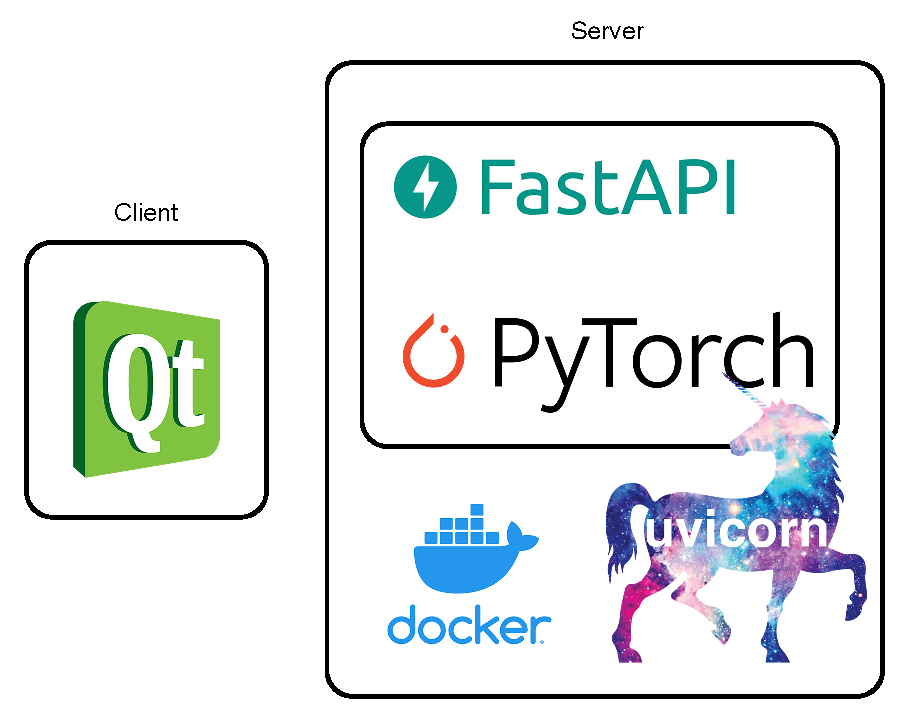
\includegraphics[height=2.5in]{content/resources/new_images/application/arch.pdf}
    \caption{Overall architecture of application}
    \label{fig:arch_app}
\end{figure}

% To prove our claim before, that our concept can easily adapt with out-of-domain
% data, we introduce an annotation tool. Back-end server that is hosted based
% on requirements of provided service. And communicate with the Graphic User
% Interface through REST API via HTTPs protocol. With separated concerns,
% each side can be developed and deployed independently. The User Interface is
% designed on QT framework. The server wrapped by Uvicorn which is an ASGI
% web server implementation for Python. All the components are wrapped by
% Docker for version compatible (figure 6.1). The application is demonstrate our
% proposed method for interactive volume organs segmentation.


To prove our claim before, that our concept can easily adapt with out-of-domain data, we introduce an annotation tool. As usual, it comprises of two separated sides, the client and the server. The back-end server is hosted based on requirements of the provided service and communicate with the  Graphic User Interface (GUI), which runs on the client machine, through REST API via HTTPs protocol. This setup potentially helps reduce the dependency between the client and server, each side can be developed and deployed independently. We use the QT framework to build a simple GUI for our application while the server is wrapped up by Uvicorn, which is an ASGI web server implementation in Python. Docker is also used to pack the whole server into a bundle for maintaining version compatibility (figure \ref{fig:arch_app}). The application is used to demonstrate our proposed method for interactive volume organs segmentation. 